\newpage
\section{改良型細径羽状筋の開発}
本章では,先行研究\cite{hasegawa}において開発された羽状筋に関する3つの課題点について,どのように解決を行ったかを述べる.
%%%%%%%%%%%%%%%%%%%%%%%%%%%%%%%%%%%%%%%%%%%%%%%%%%%%%%%%%
\subsection{先行研究で確認された課題}
先行研究\cite{hasegawa}で開発された歩脚ロボットで脚の開閉動作を確認することができたが,以下のような3つの課題が見つかった.
\begin{enumerate}
  \item 細径MPA端部の締結方法が煩雑で,細径MPAを完成させるまでに時間かかり,また締結部から空気漏れが生じる可能性が高い
  \item シリコンゴムチューブと編組チューブの間に隙間が生じてしまい収縮率が低下する
  \item 細径MPAの根元の部品が角度を固定されていて,腱の引き込みを妨げている
\end{enumerate}
以上の3つの課題の解決するために4.1,4.2,4.3で示す対策を講じた.
%%%%%%%%%%%%%%%%%%%%%%%%%%%%%%%%%%%%%%%%%%%%%%%%%%%%%%%%%
\subsection{課題1:細径MPAの制作方法の改良}
先行研究\cite{hasegawa}の細径MPA締結方法を図\ref{fig:MPA_tanbu_1}に示す.
先行研究\cite{hasegawa}では,細径MPAを構成するシリコンチューブとスリーブを端部で糸で縛り接着剤で固定する方式を採用していた.
しかし,この方法では作製するのに時間がかかる.また,空気漏れが発生しやすく,細径MPAの製作には技術と練度が必要となる.
そこで本研究では,図\ref{fig:MPA_tanbu_2}のように細径MPA端部部品とOリングを用いた新しい細径MPA作製方法を開発した.
新型細径MPAの作製手順を以下に示す.従来の細径MPA作製方法を用いると作製時間が約20分なのに対し,本研究の作製方法では約10分で作製することが可能であり,
空気漏れなど、作成後に確認される不具合の発生確率も大幅に低減した.
先行研究と本研究ではPPX(瞬間接着剤) (セメダイン社製,CA-522)を用いて細径MPAを作成した.
%\vspace{3mm}
\begin{enumerate}
  \item 図\ref{fig:MPA_tanbu_2}\subref{fig:MPA_tanbu_2_2}のようにゴムチューブを端部部品の溝部分に差し込み,差し込んだ隙間に接着剤を塗布する
  \item 接着剤が乾いたら,図\ref{fig:MPA_tanbu_2}\subref{fig:MPA_tanbu_2_1}のようにゴムチューブと端部部品をスリーブで包む
  \item 図\ref{fig:MPA_tanbu_2_1}のように図\ref{fig:MPA_tanbu_2}\subref{fig:MPA_tanbu_2_2}中のOリング固定溝にはまるようにOリングを配置する
  \item 端部部品,スリーブとOリングを固定するために接着剤を塗布する
\end{enumerate}
%%%%%%%%%%%%%%%%%%%%%%%%%%%%%%%%%%%%%%%%%%%%%%%%%%%%%%%%%
\begin{figure}[htbp]
  %
  \begin{minipage}{0.49\hsize}
    \centering  
    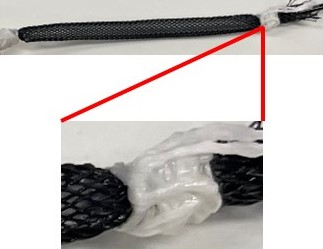
\includegraphics[scale=0.6]{image/MPA_tanbu_1_1.jpg}
    \subcaption{旧型細径MPA外観}
    \label{fig:MPA_tanbu_1_1}
  \end{minipage}
  %
  \begin{minipage}{0.5\hsize}
    \centering
    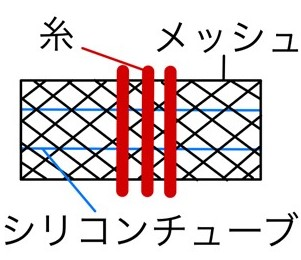
\includegraphics[scale=0.6]{image/MPA_tanbu_1_2.jpg}
    \subcaption{旧型細径MPA模式図}
    \label{fig:MPA_tanbu_1_2}
  \end{minipage}
  %
  \caption{先行研究で用いられた旧型細径MPAおよび作製方法}
  \label{fig:MPA_tanbu_1}
\end{figure}
%
\begin{figure}[htbp]
  \begin{minipage}{0.49\hsize}
    \centering
    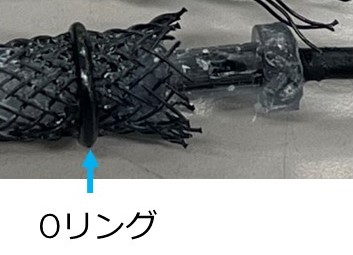
\includegraphics[scale=0.6]{image/MPA_tanbu_2_2.jpg}
    \subcaption{新型細径MPA外観}
    \label{fig:MPA_tanbu_2_1}
  \end{minipage}
  %
  \begin{minipage}{0.499\hsize}
    \centering  
    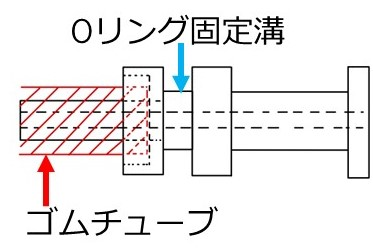
\includegraphics[scale=0.6]{image/MPA_tanbu_2_1.jpg}
    \subcaption{新型細径MPA模式図}
    \label{fig:MPA_tanbu_2_2}
  \end{minipage}
  %
  
  \begin{minipage}{0.49\hsize}
    \vspace{5mm}
    \centering  
    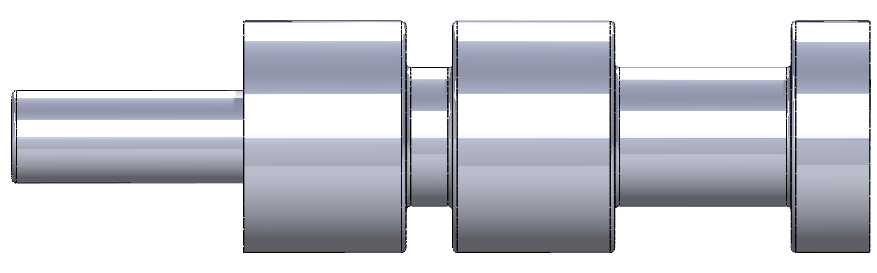
\includegraphics[scale=0.3]{image/tanbubuhin.png}
    \vspace{7mm}
    \subcaption{新型細径MPAのCADの様子(横)}
    \label{fig:MPA_tanbu_2_3}
  \end{minipage}
  %
  \begin{minipage}{0.49\hsize}
    \vspace{5mm}
    \centering  
    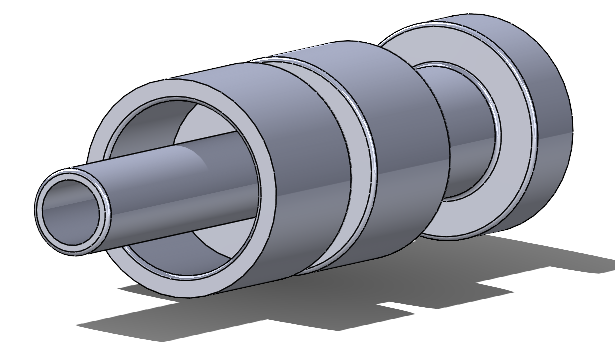
\includegraphics[scale=0.3]{image/MPA_cap.png}
    \subcaption{新型細径MPAのCADの様子(断面)}
    \label{fig:MPA_tanbu_2_4}
  \end{minipage}
  \caption{本研究で用いた新型細径MPAおよび作製方法}
  \label{fig:MPA_tanbu_2}
\end{figure}
%%%%%%%%%%%%%%%%%%%%%%%%%%%%%%%%%%%%%%%%%%%%%%%%%%%%%%%%%
\clearpage
\subsection{課題2:細径MPAの収縮率向上}
市販に売られている編組チューブは,図\ref{fig:messhu_henka}\subref{fig:messhu_1}のように断面が平たく折癖がついている.
その状態の編組チューブを用いて細径MPAを作成すると,図\ref{fig:MPA_henka}\subref{fig:MPA_1}のようにシリコンゴムチューブ(青色)と編組チューブの間に隙間が生じてしまう.
これにより,自身の径方向に膨張し軸方向に収縮する細径MPAでは収縮率が低下してしまう.
そこで本研究では,細径MPAの収縮性能を高めるために編組チューブを熱可塑変化させる加工を行い,径を小さくすることで収縮率の向上を試みた.
大まかな作成方法を図\ref{fig:messhu_method}に示す.
図\ref{fig:messhu_method}中\textcircled{\scriptsize 1}に示した物品が作製に必要なもので左から以下の通りである.
%
\begin{itemize}
  \item マスキングテープ テープ幅 15mm (モノタロウ社製,15)
  \item 編組チューブ ほつれにくいタイプ 1×5(最小径×最大径) (モノタロウ社製,6993303)
  \item ステンレス丸棒 $\phi$ 2mm (モノタロウ社製,1378)
  \item ホットプレート (山善社製,YHA-W102)
\end{itemize}
%
加工の手順を以下に示す.
\vspace{3mm}
\begin{enumerate}
  \item まず初めに,編み込みチューブをステンレス棒よりも 3cm程短い範囲で任意の長さに切る
  \item 編み込みチューブにステンレス棒を差し込む(図中\textcircled{\scriptsize 2})
  \item 編み込みチューブの内径がステンレス棒の外径になるようにマスキングテープで巻いて固定する(図中\textcircled{\scriptsize 3})
  \item ホットプレートを 180℃まで温めて,編み込みチューブ全体に熱が伝わるように転がしながら3分間温める(図中\textcircled{\scriptsize 4})
  \item 全体を冷水に漬けて,3分間ほど熱をとる(図中\textcircled{\scriptsize 5})
  \item 粗熱が取れたらマスキングテープを外して完成
\end{enumerate}
熱可塑変化させていない編組チューブを図\ref{fig:messhu_henka}\subref{fig:messhu_1},熱可塑変化させた編組チューブを図\ref{fig:messhu_henka}\subref{fig:messhu_2}に示す.
熱可塑変化させていない編組チューブは折癖があり,断面が平たいのに対し.熱可塑変化した編組チューブは折癖が取れ,断面が円形になっている.
この熱可塑変化させた編組チューブを用いて細径MPAを作製したものを図\ref{fig:MPA_henka}\subref{fig:MPA_2}に示す.
図\ref{fig:MPA_henka}\subref{fig:MPA_1}と比べるとシリコンチューブ(青色)と編組チューブの間が狭くなっていることがわかる.
熱可塑変化させたメッシュを用いて作製した新型細径MPAの収縮性能の変化を調べたところ,
熱可塑変化させていないメッシュを用いた旧型細径MPAの収縮率が 16%なのに対して,新型細径MPAの収縮率は 20%と向上したことを確認することができた.
%%%%%%%%%%%%%%%%%%%%%%%%%%%%%%%%%%%%%%%%%%%%%%%%%%%%%%%%%
%
\begin{figure}[htbp]
  %
  \begin{minipage}{0.49\hsize}
    \centering  
    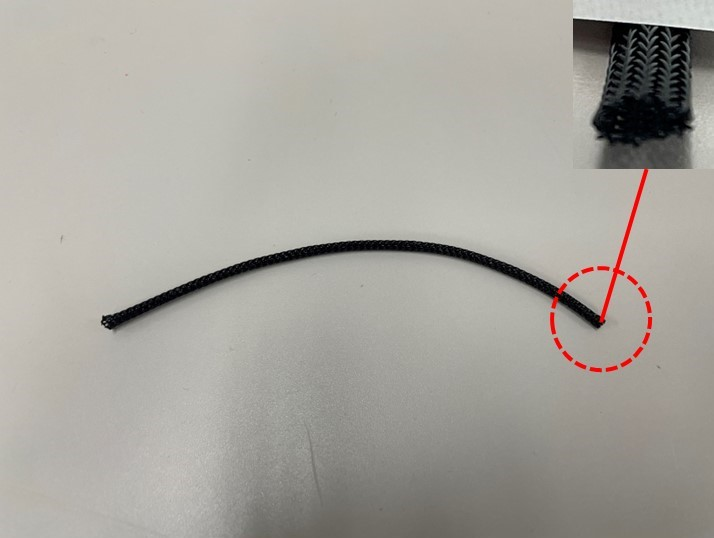
\includegraphics[scale=0.25]{image/messhu_hikaku_1.jpg}
    \subcaption{変化前}
    \label{fig:messhu_1}
  \end{minipage}
  %
  \begin{minipage}{0.49\hsize}
    \centering
    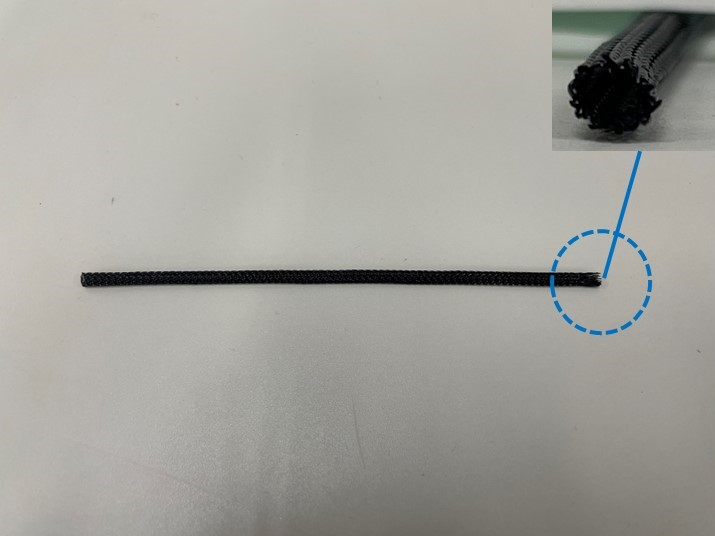
\includegraphics[scale=0.25]{image/messhu_hikaku_2.jpg}
    \subcaption{変化後}
    \label{fig:messhu_2}
  \end{minipage}
  %
  \caption{メッシュの熱可塑変化の様子}
  \label{fig:messhu_henka}
\end{figure}
%
\begin{figure}[htbp]
  %
  \begin{minipage}{0.49\hsize}
    \centering  
    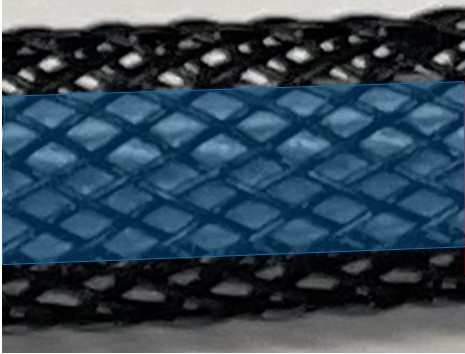
\includegraphics[scale=0.4]{image/hikaku_MPA_1.jpg}
    \subcaption{変化前}
    \label{fig:MPA_1}
  \end{minipage}
  %
  \begin{minipage}{0.49\hsize}
    \centering
    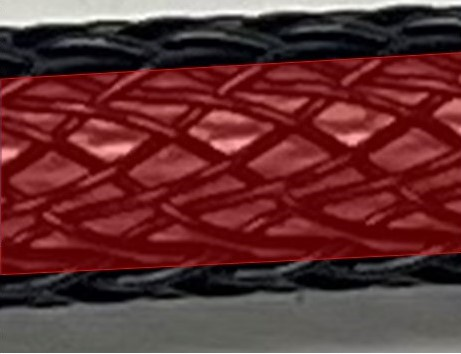
\includegraphics[scale=0.4]{image/hikaku_MPA_2.jpg}
    \subcaption{変化後}
    \label{fig:MPA_2}
  \end{minipage}
  %
  \caption{細径MPAの熱可塑変化の様子}
  \label{fig:MPA_henka}
\end{figure}
%
\begin{figure}[htbp]
  \centering
  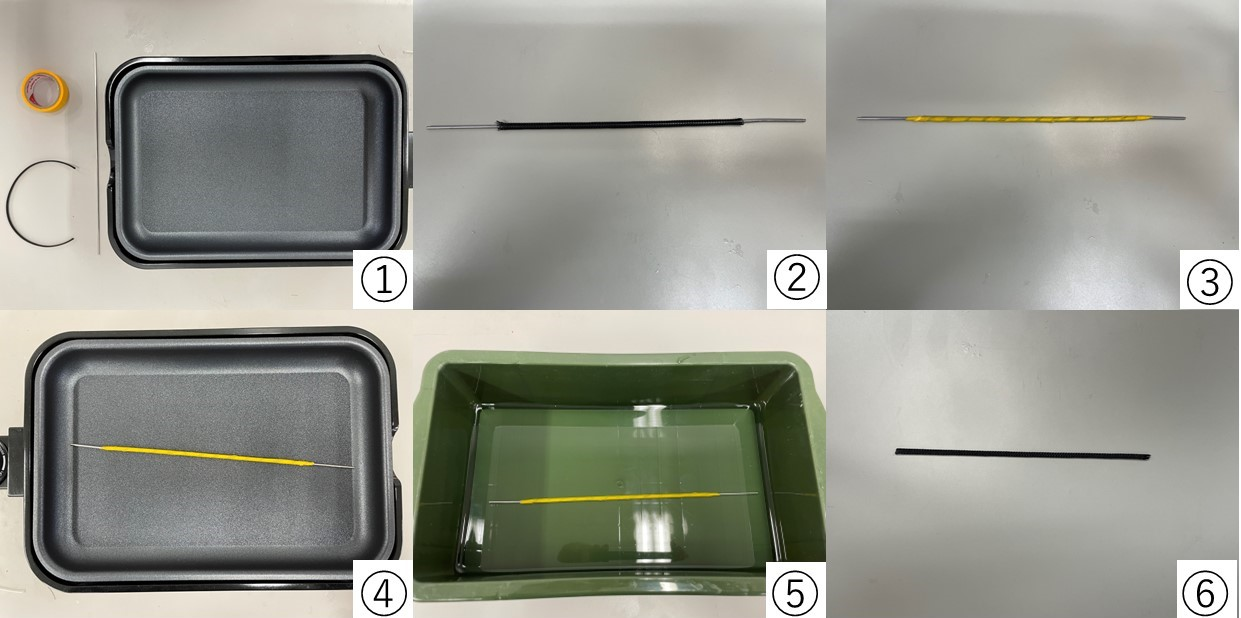
\includegraphics[scale=0.4]{image/messhu_tejyun.jpg}
  \caption{熱可塑変化の手順}
  \label{fig:messhu_method}
\end{figure}
%
%%%%%%%%%%%%%%%%%%%%%%%%%%%%%%%%%%%%%%%%%%%%%%%%%%%%%%%%%
\clearpage
\subsection{課題3:羽状角の変化に対する対応}
細径MPAを用いた羽状筋による腱の引き込みを模式図にしたものを図\ref{fig:ujyoukin_moshiki}に示す.
細径MPAが収縮することにより,腱が長手方向(赤い矢印の方向)へ引っ張られる.
このとき,腱と細径MPAのなす角(羽状角)は収縮前後で変化するため,細径MPAの腱および外殻への付着点(図\ref{fig:ujyoukin_moshiki}中赤点)は回転自由度を持つ必要がある.
しかし,先行研究\cite{hasegawa}で作製された細径MPAを用いた羽状筋では,細径MPA端部の部品の角度が固定されていた.(図\ref{fig:ujyoukin_kako}\subref{fig:ujyoukin_real_kako})
そのため,細径MPAが収縮した際に細径MPA自身が折れ曲がるように変形してしまい,腱を十分に引くことができず,関節可動域が狭くなる原因の1つとなっていた.

そこで本研究では細径MPAの端部に回転自由度を持たせる構造を考案した.図\ref{fig:tanbu_parts_new}に構造を示す.
図\ref{fig:tanbu_parts_new}\subref{fig:tanbu_parts}に示すように,MPA端部部品(部品\textcircled{\scriptsize 3})の軸部分を両側から挟むように,
部品\textcircled{\scriptsize 1}\textcircled{\scriptsize 2}を取り付ける.
部品\textcircled{\scriptsize 1}\textcircled{\scriptsize 2}にはMPA端部部品の軸と直行する向きに穴があけてある.
組み立てたものを土台部品にとり付け,部品\textcircled{\scriptsize 1}\textcircled{\scriptsize 2}を左右からネジで固定する(図\ref{fig:tanbu_parts_new}\subref{fig:MPA_tanbu_3_2}).
このとき,ネジの先端が部品\textcircled{\scriptsize 1}\textcircled{\scriptsize 2}の穴部にはまることで,このネジが回転軸となり細径MPA端部が自由度を持つことができる.
また細径MPAの外殻側は圧縮空気を供給するために中空状になっており,そこへ$\phi$ 3mmのポリウレタンチューブを挿入して接着剤で固定する.
また土台部品も圧縮空気を供給するための流路が内部に設けてあり,ポリウレタンチューブの他方はそちらに挿入して接着剤で固定する.
図\ref{fig:tanbu_parts_new}\subref{fig:MPA_tanbu_3_2}に実際に細径MPAを土台に組付けた様子を示す.
%%%%%%%%%%%%%%%%%%%%%%%%%%%%%%%%%%%%%%%%%%%%%%%%%%%%%%%%%
%
\begin{figure}[htbp]
  \centering
  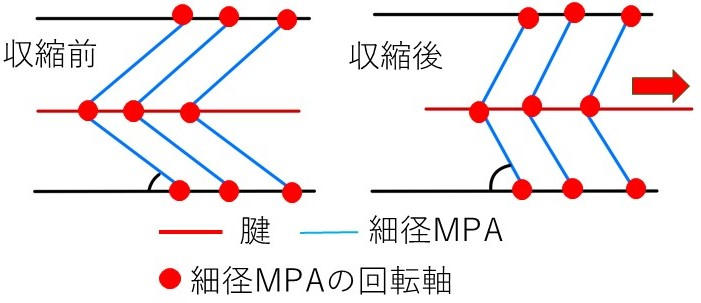
\includegraphics[scale=0.5]{image/ujyoukin.jpg}
  \caption{羽状筋の動作の模式図}
  \label{fig:ujyoukin_moshiki}
\end{figure}
%
\begin{figure}[htbp]
  %
  \begin{minipage}{0.49\hsize}
    \centering  
    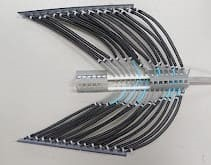
\includegraphics[scale=0.9]{image/syuseki_1.JPG}
    \subcaption{旧型羽状筋}
    \label{fig:ujyoukin_real_kako}
  \end{minipage}
  %
  \begin{minipage}{0.49\hsize}
    \centering
    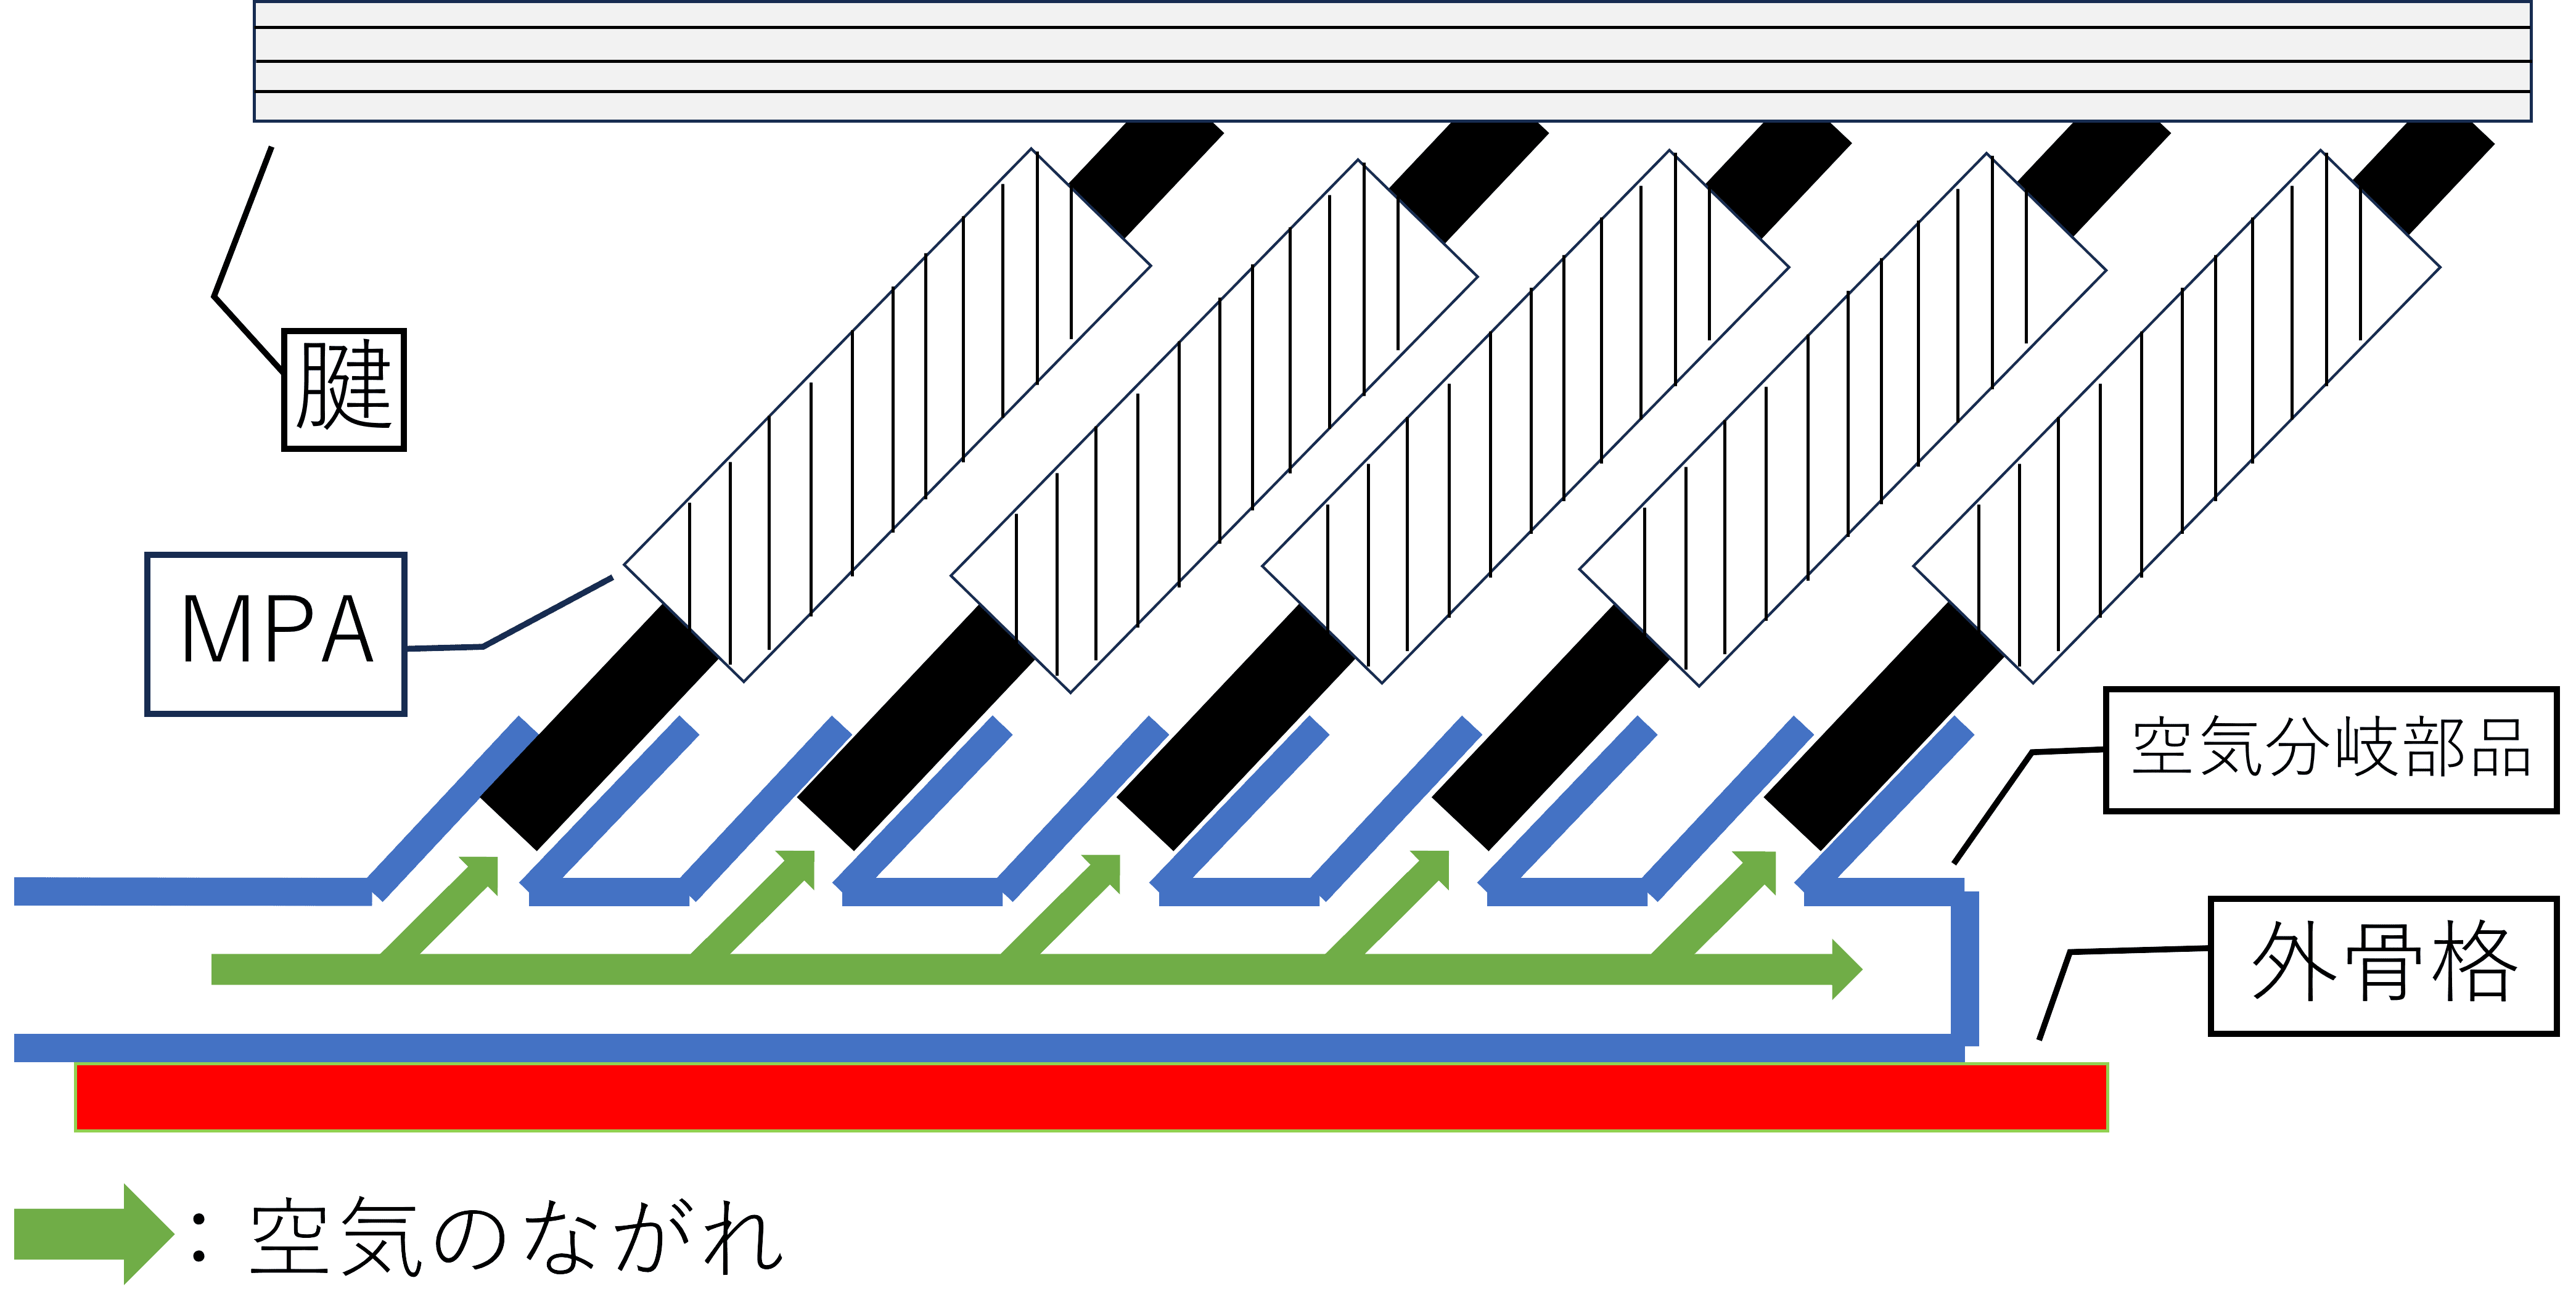
\includegraphics[scale=0.04]{image/air_moshiki.png}
    \subcaption{模式図}
    \label{fig:ujyoukin_moshiki_kako}
  \end{minipage}
  %
  \caption{先行研究で開発された羽状筋}
  \label{fig:ujyoukin_kako}
\end{figure}
%
\begin{figure}[htbp]
  %
  \begin{minipage}{0.45\hsize}
    \centering  
    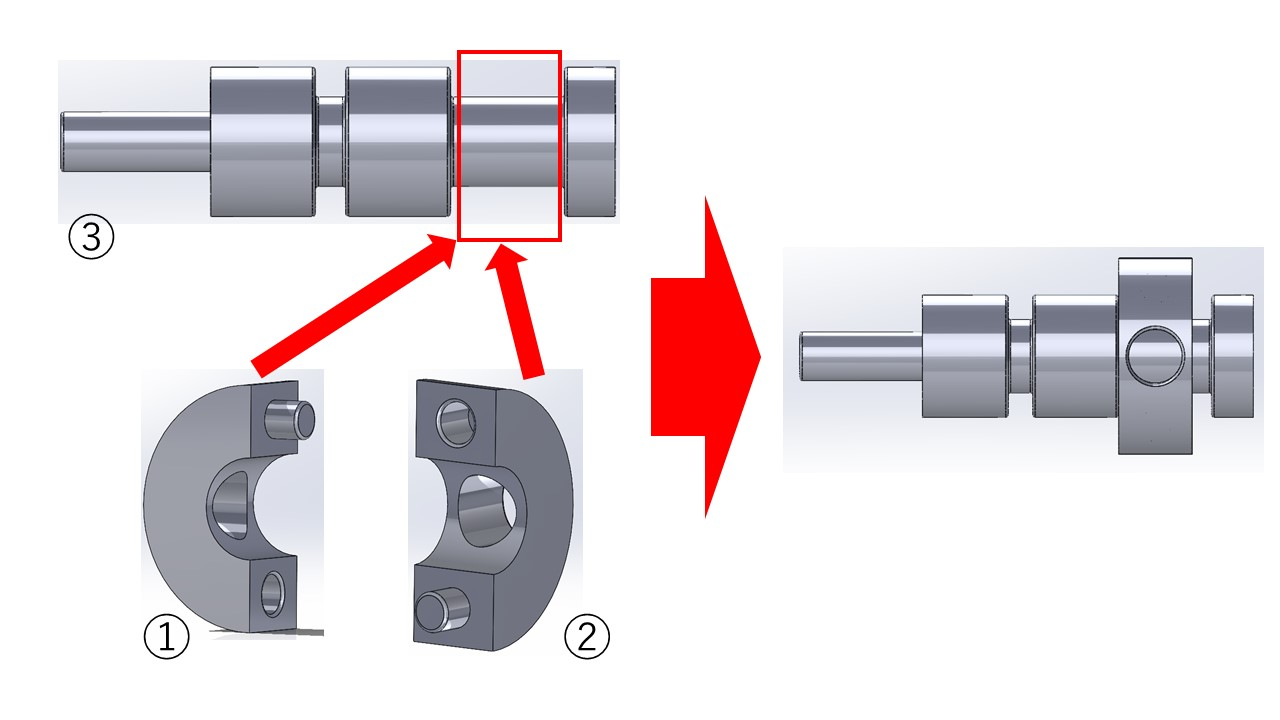
\includegraphics[scale=0.2]{image/tanbu_parts.jpg}
    \subcaption{組み立て方法}
    \label{fig:tanbu_parts}
  \end{minipage}
  %
  \begin{minipage}{0.49\hsize}
    \centering
    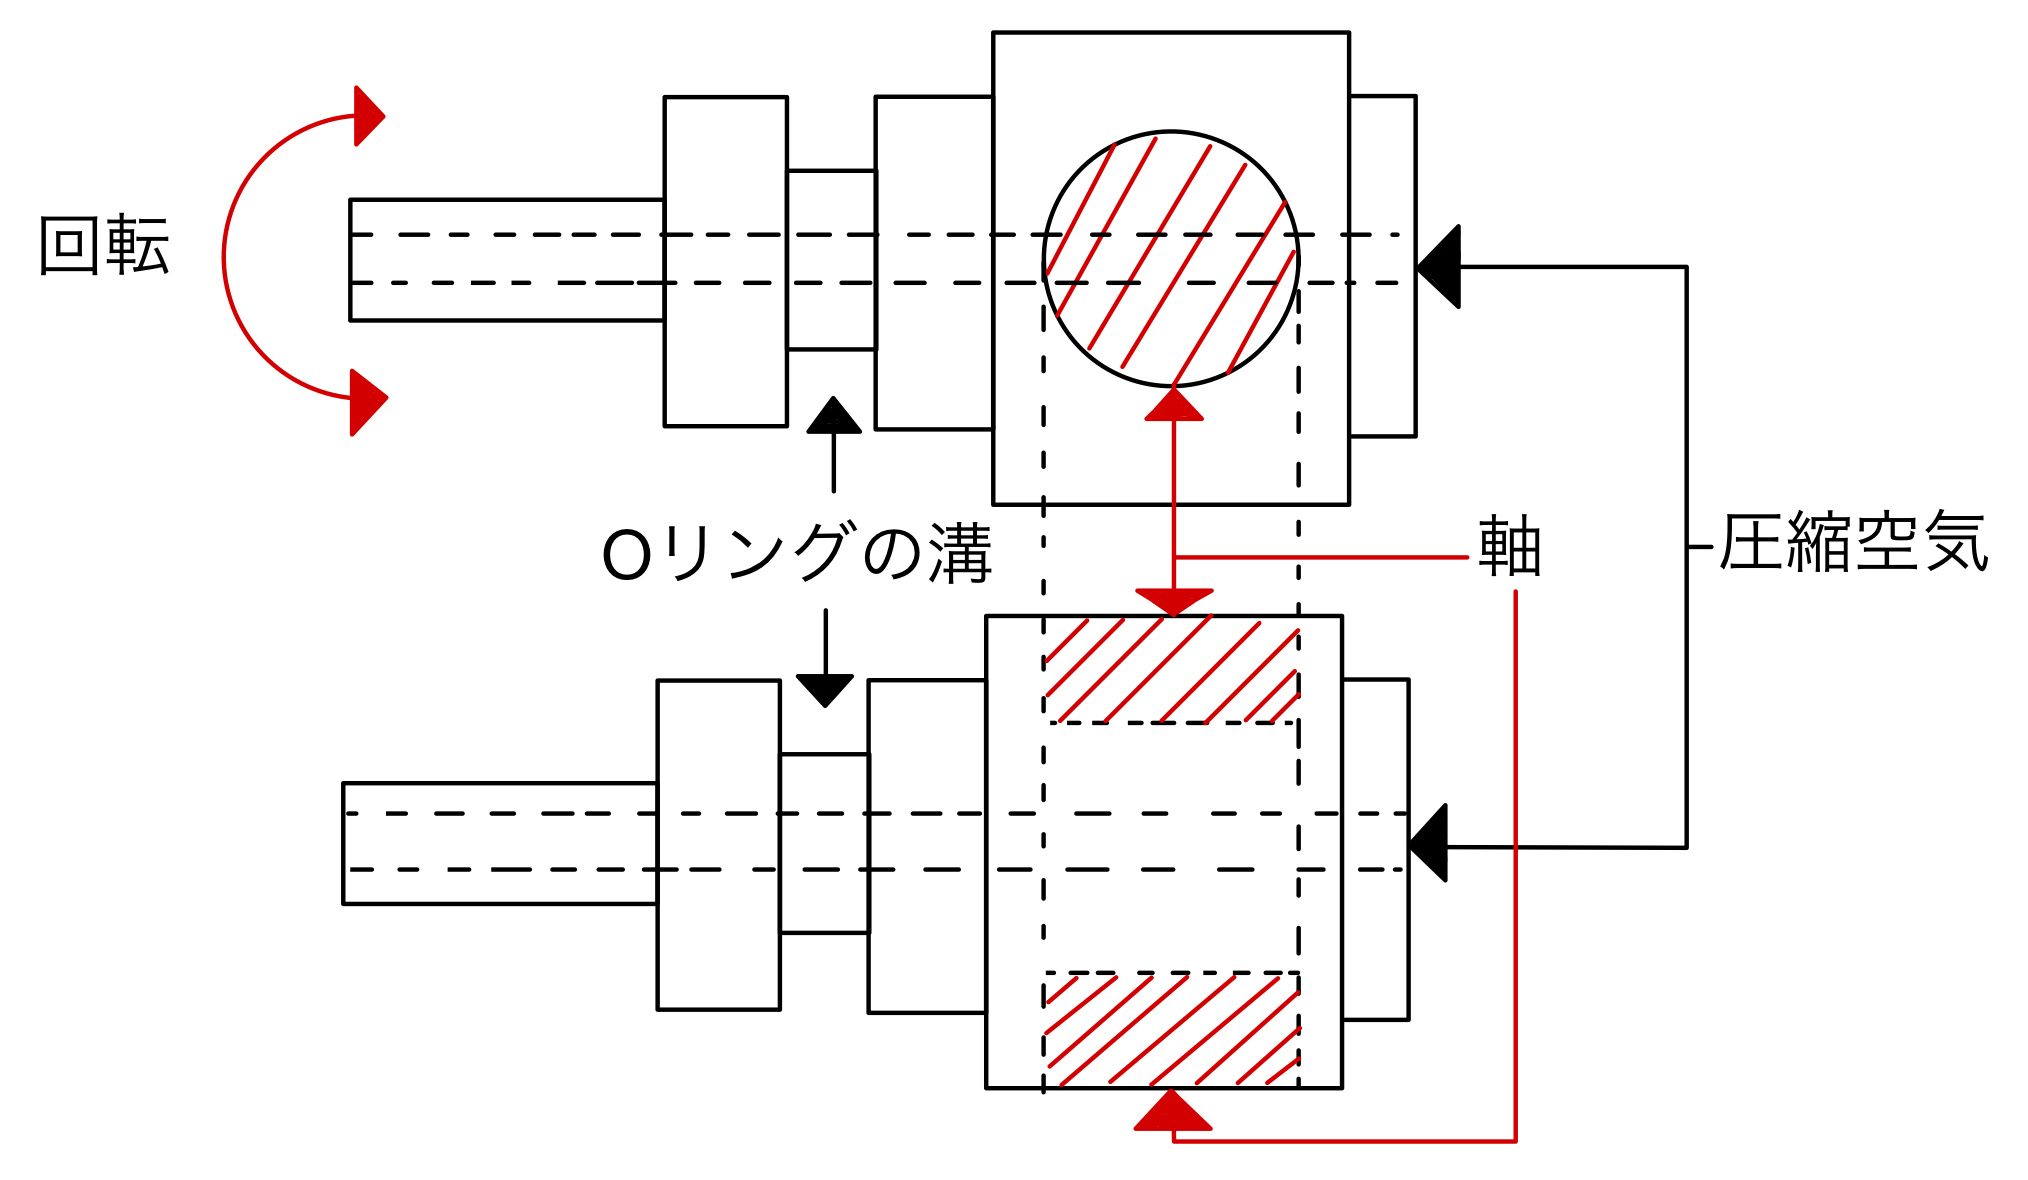
\includegraphics[scale=0.085]{image/MPA_irast.jpg}
    \subcaption{模式図}
    \label{fig:tanbu_moshikizu}
  \end{minipage}
  %
  \begin{minipage}{0.49\hsize}
    \centering
    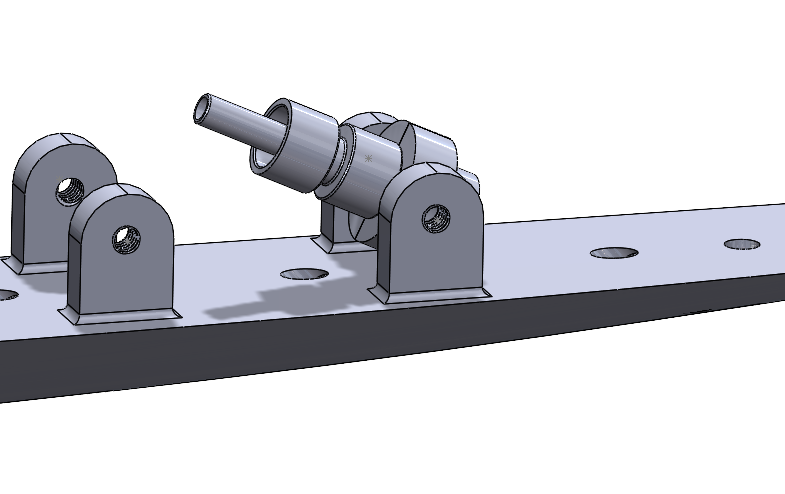
\includegraphics[scale=0.2]{image/asenburi_tanbu.png}
    \subcaption{新型細径MPAのCADの様子}
    \label{fig:MPA_tanbu_3_1}
  \end{minipage}
  %
  \begin{minipage}{0.49\hsize}
    \centering  
    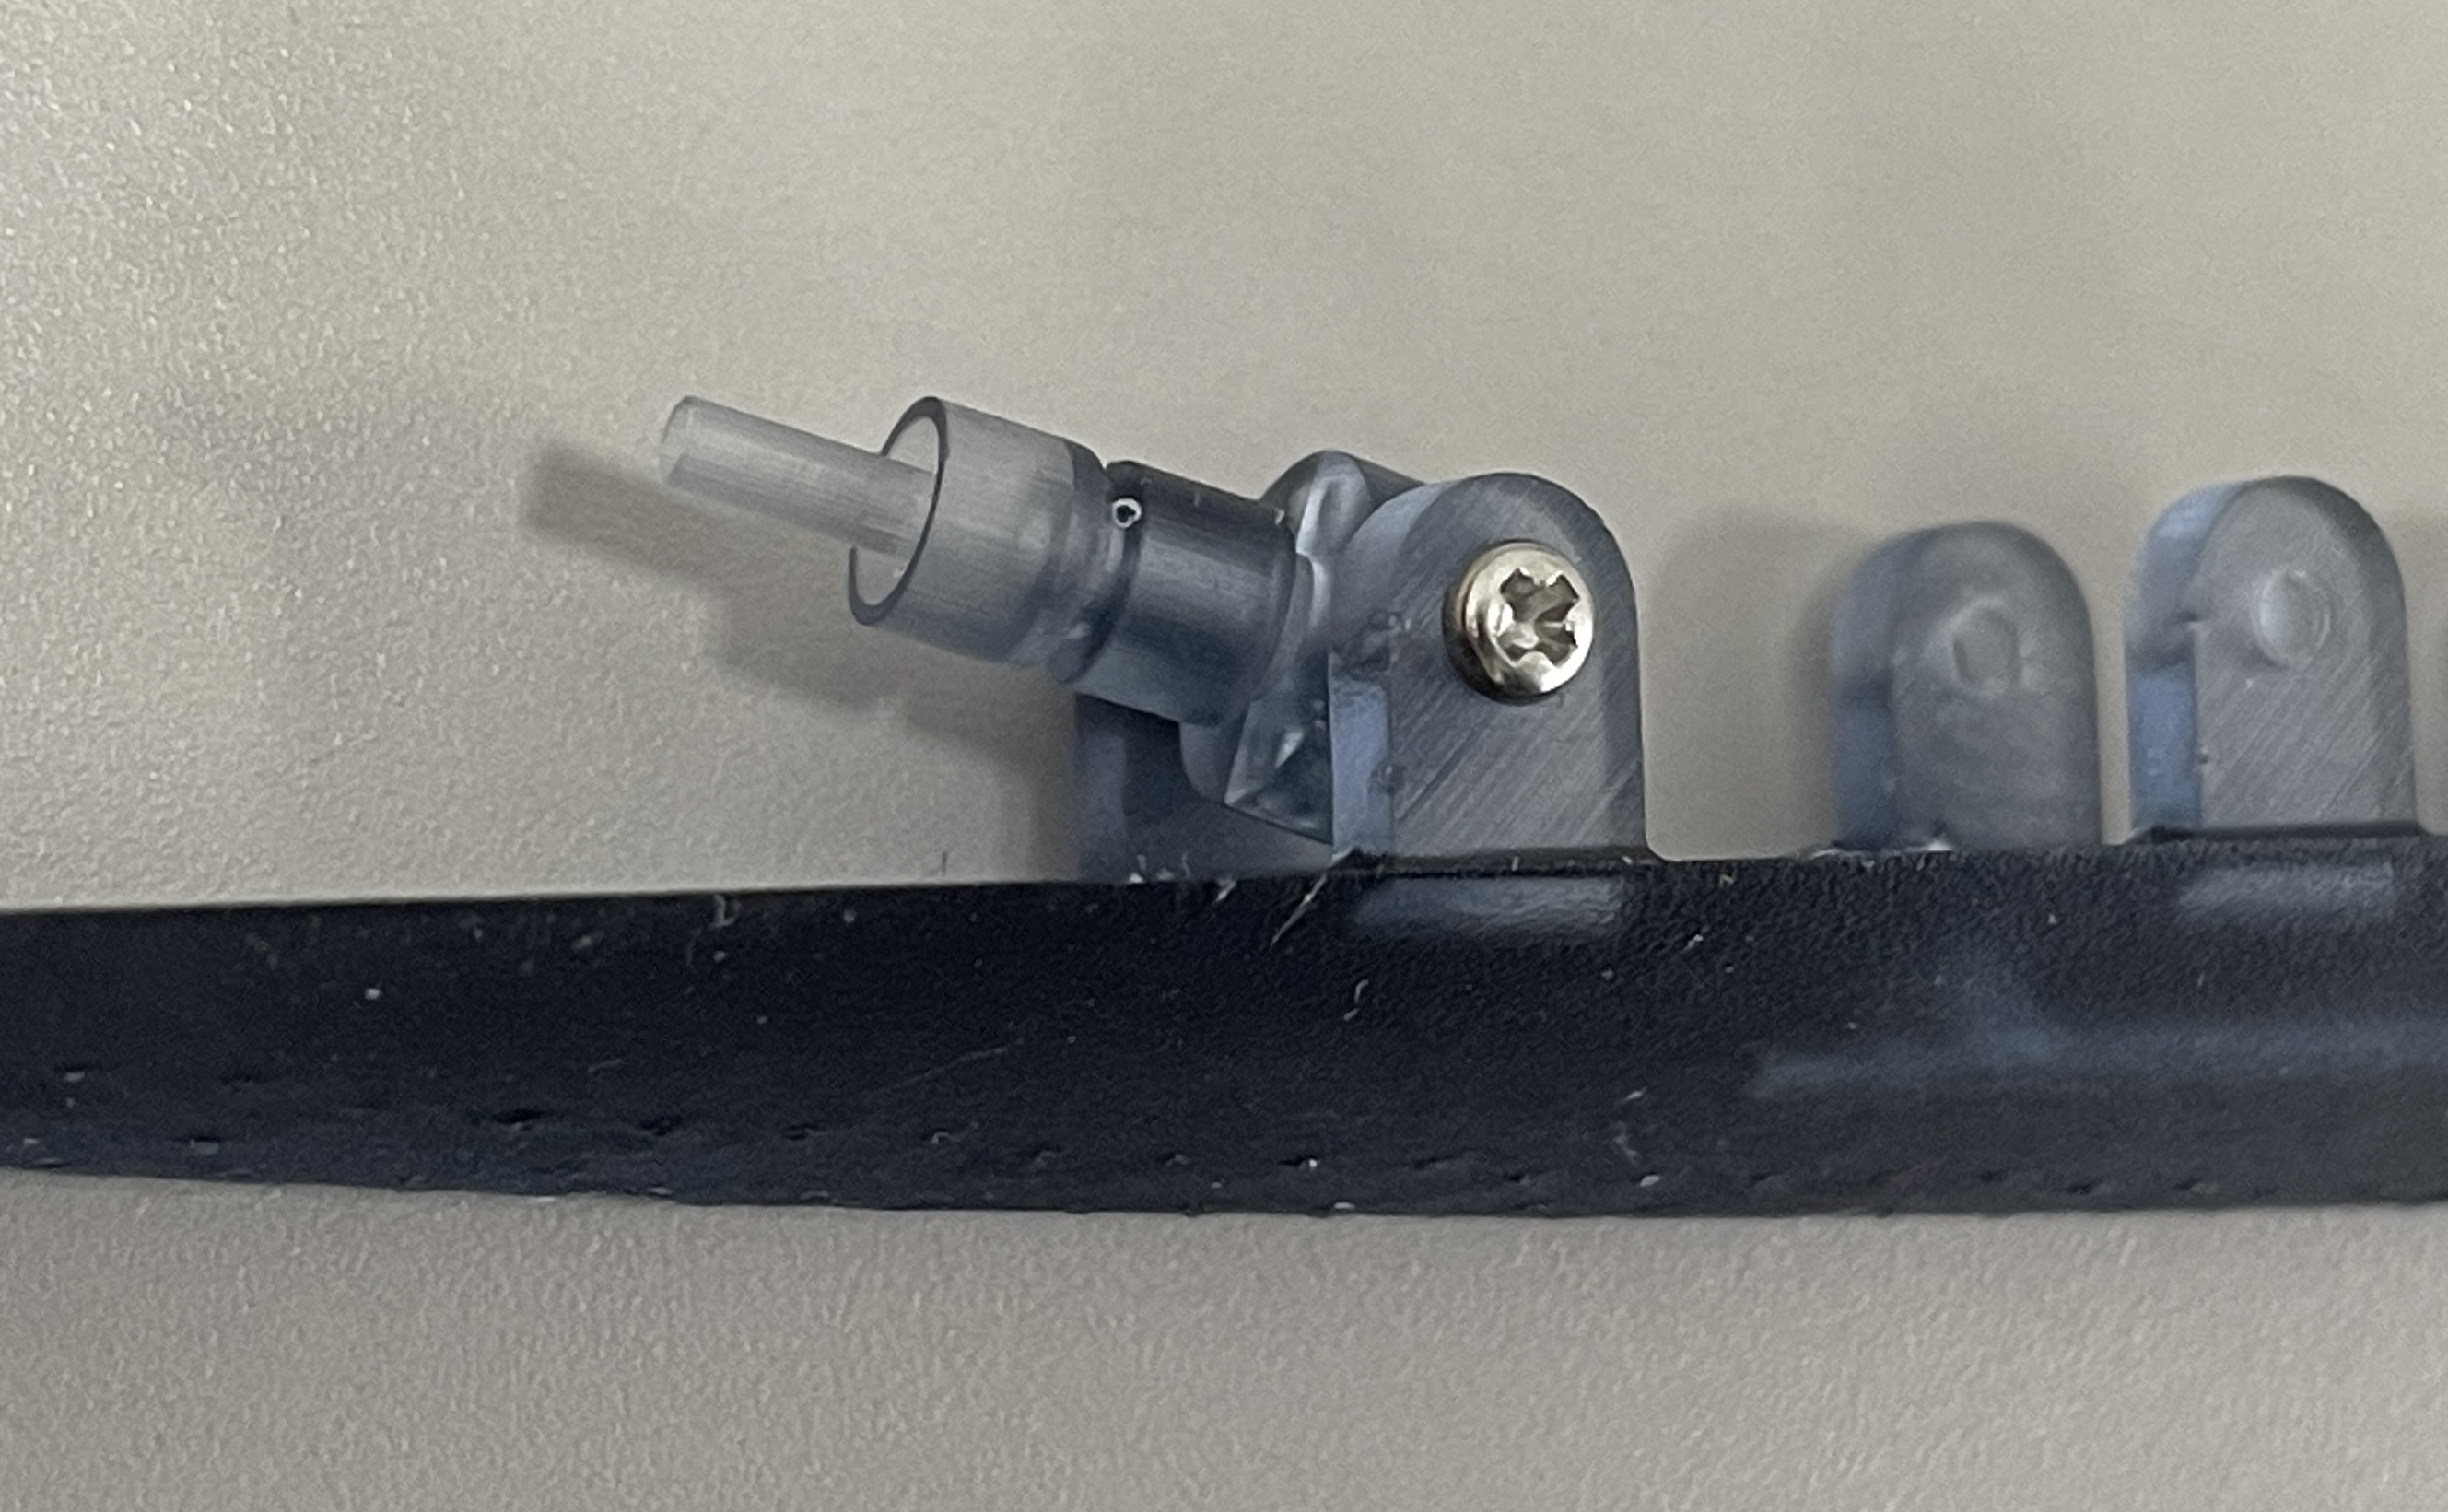
\includegraphics[scale=0.2]{image/real_tanbu.jpg}
    \subcaption{新型細径MPAの固定の様子}
    \label{fig:MPA_tanbu_3_2}
  \end{minipage}
  \caption{先行研究で開発された羽状筋}
  \label{fig:tanbu_parts_new}
\end{figure}
%%%%%%%%%%%%%%%%%%%%%%%%%%%%%%%%%%%%%%%%%%%%%%%%%%%%%%%%%
\subsection{改良型細径羽状筋}
前述した先行研究の課題1,2,3の解決方法を取り入れて開発した改良型細径空圧羽状筋を図\ref{fig:ujyoukin_new}に示す.
図\ref{fig:ujyoukin_new}中の腱は柔軟な素材であるTPUを用いてFDM方式3Dプリンターで,外殻部分はPLAを用いてFDM方式の3Dプリンターで,
細径MPA固定部品は光造形方式の3Dプリンターでそれぞれ作成した.
3.2で述べたように,圧縮空気印加前の羽状角を 20度かつすべての細径MPAの長さは等しいという条件のもと,可能な限り外骨格内部に細径MPAを配置した.
また外殻の幅の制約から,すべての節で屈筋伸筋は一列ずつとした.
本研究で開発した各節の羽状筋を図\ref{fig:ujyou_new_real}に示す.
長節においては屈筋伸筋ともに上下に7本ずつ,7対14筋能状筋とした.
同様に前節は4対8筋とした.腕節では屈筋伸筋ともに腱の上側が5本,下側が4本の非対称な羽状筋とした.
これは可能な限り空間内に多数の細径MPAを配置し,腱を引き込む力を大きくするためである.
%%%%%%%%%%%%%%%%%%%%%%%%%%%%%%%%%%%%%%%%%%%%%%%%%%%%%%%%%
%
\begin{figure}[htbp]
  \centering
  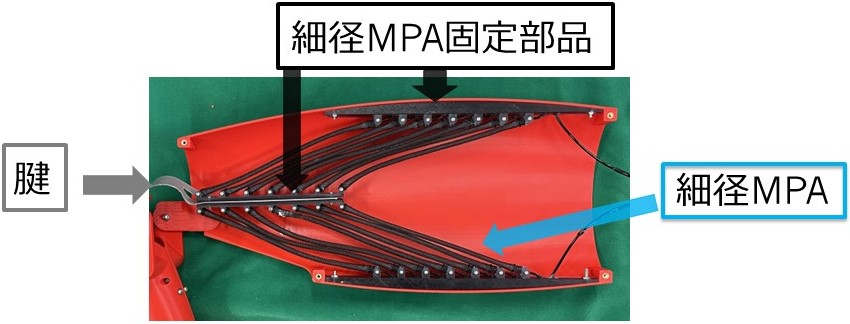
\includegraphics[scale=0.65]{image/uyjoukin_new.jpg}
  \caption{改良型細径空圧羽状筋}
  \label{fig:ujyoukin_new}
\end{figure}
%
\begin{figure}[ht]
  %
  \begin{minipage}[b]{0.45\hsize}
    \centering  
    \includegraphics[scale=0.2]{image/chousetu_MPA.jpg}
    \subcaption{長節の羽状筋の様子}
    \label{fig:chousetu_MPA_haichi}
  \end{minipage}
  %
  \begin{minipage}[b]{0.49\hsize}
    \centering
    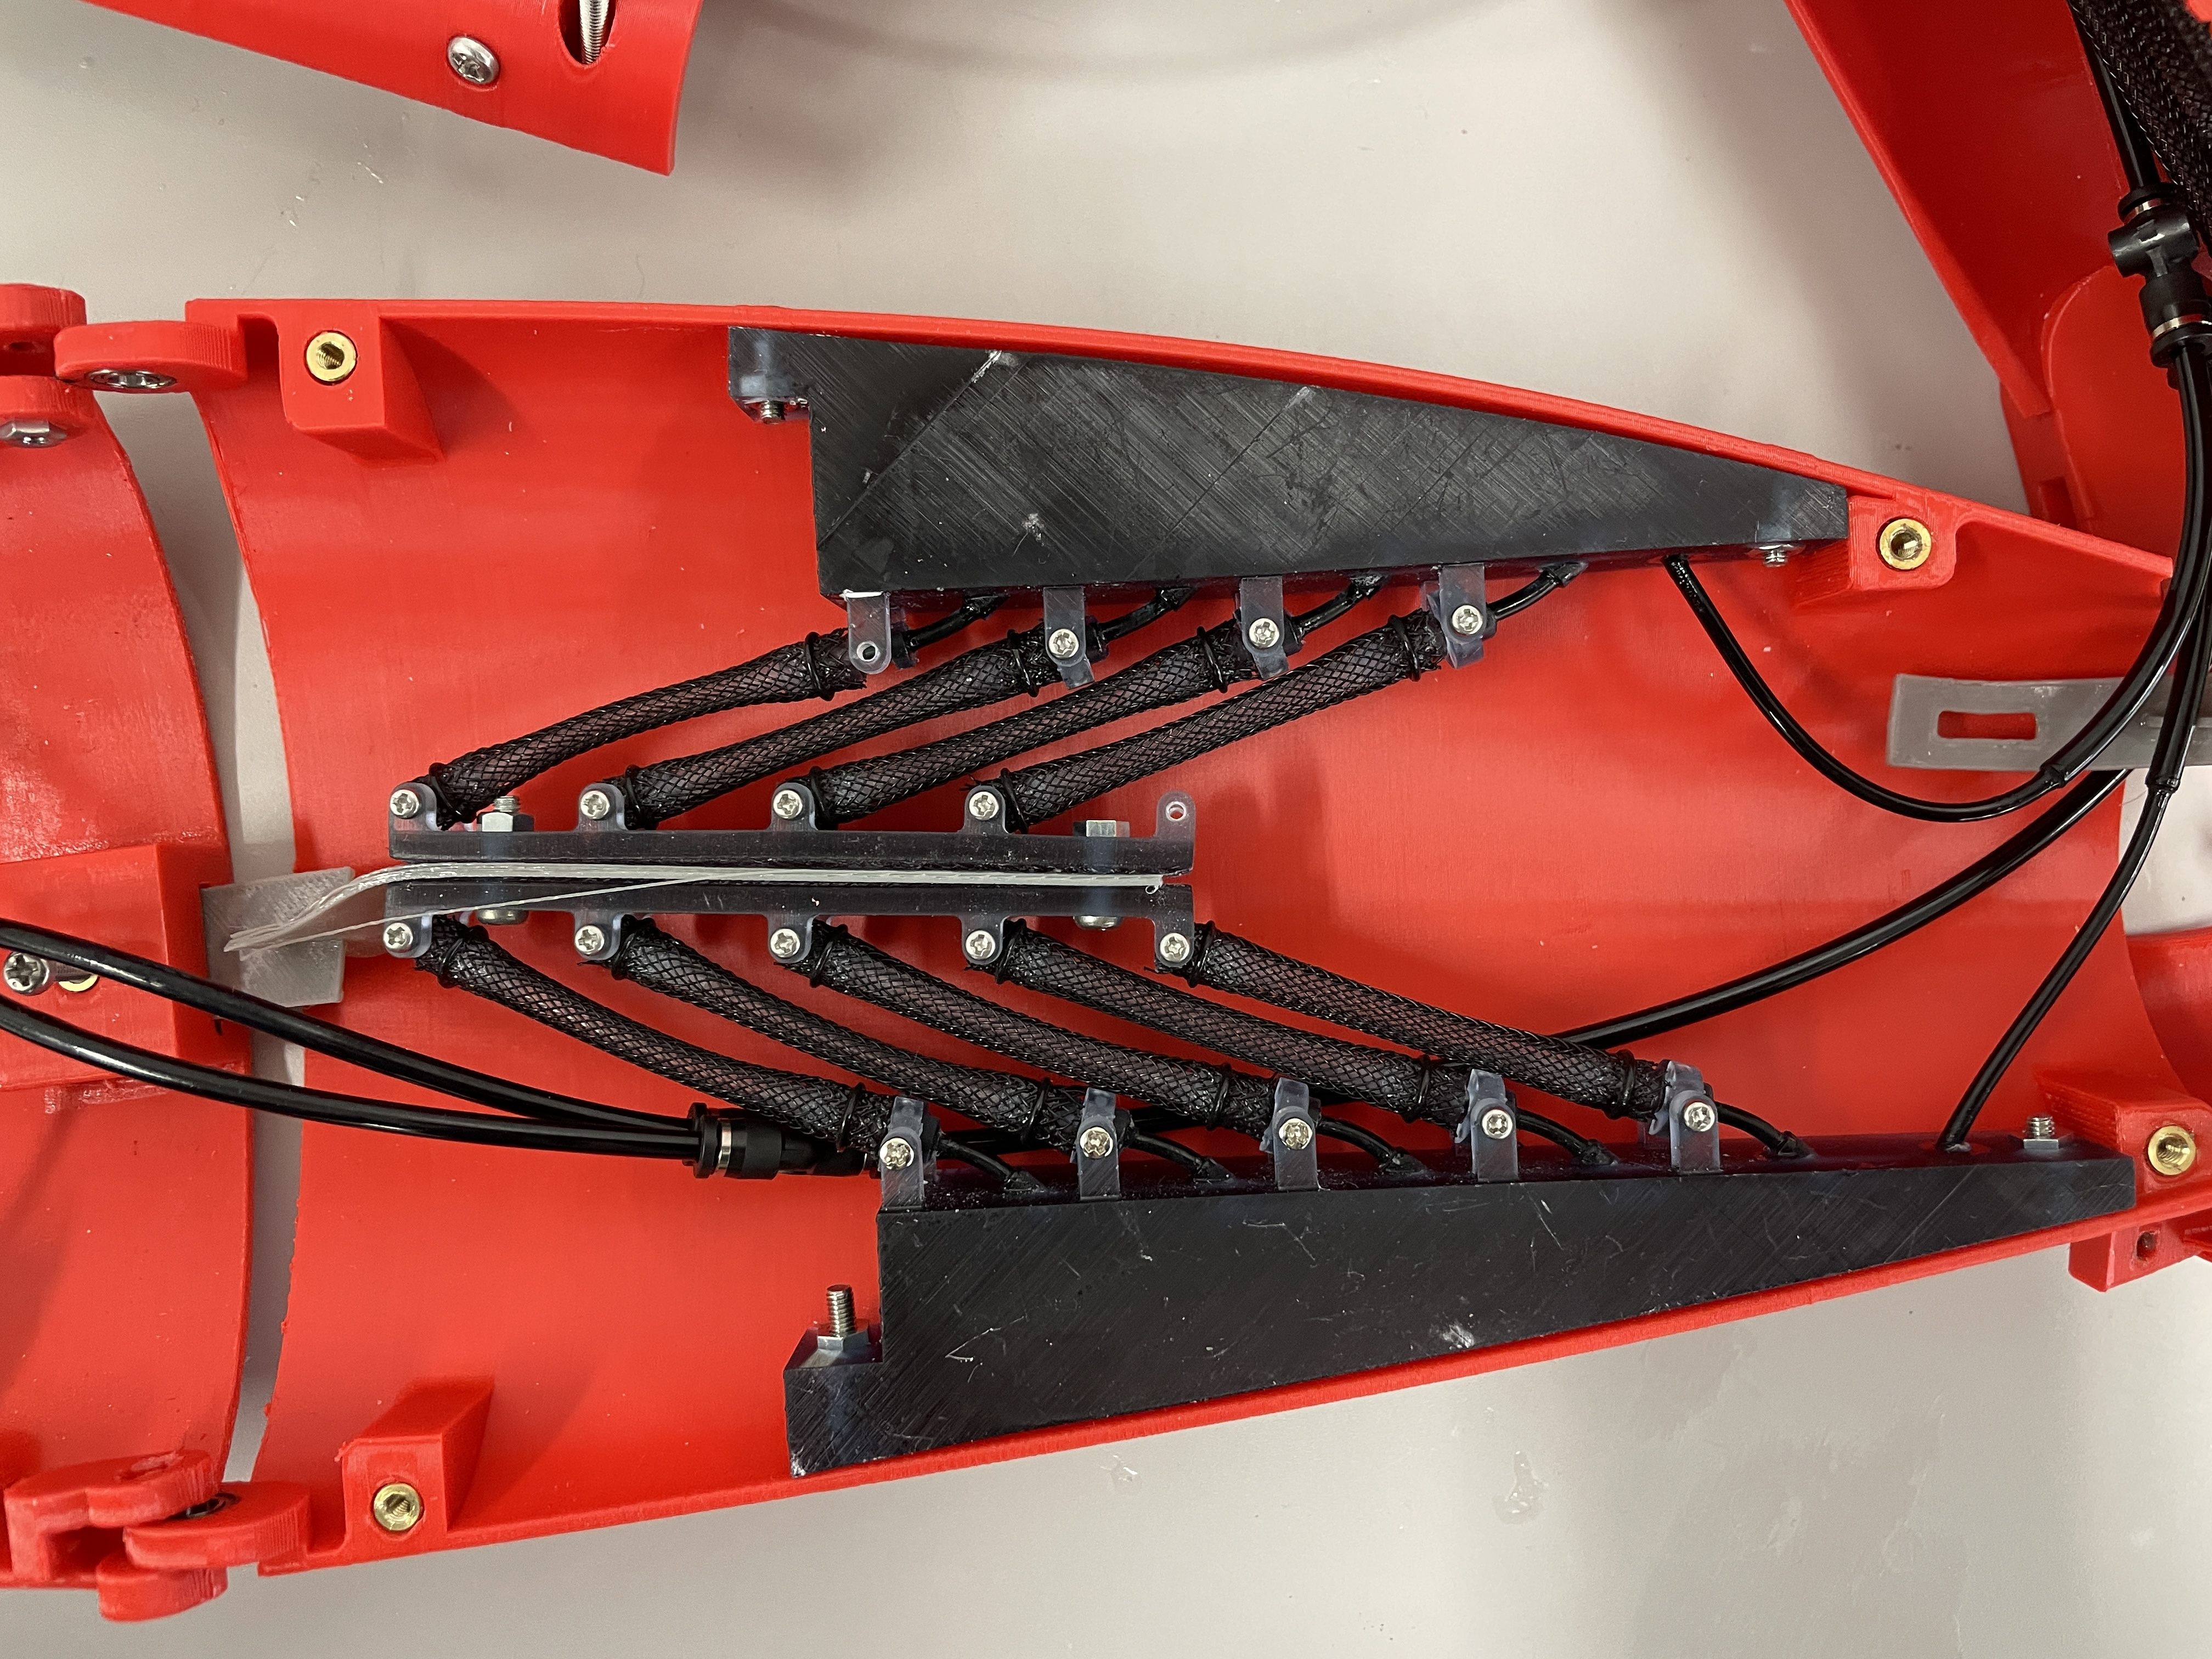
\includegraphics[scale=0.05]{image/wansetu_MPA.jpg}
    \subcaption{腕節の羽状筋の様子}
    \label{fig:wansetu_MPA_haichi}
  \end{minipage}
  %
  \begin{minipage}[b]{1\hsize}
    \centering
    \includegraphics[scale=0.25]{image/zensetu_MPA.jpg}
    \subcaption{前節の羽状筋の様子}
    \label{fig:zensetu_MPA_haichi}
  \end{minipage}
  \caption{本研究で開発した歩脚ロボットの羽状筋}
  \label{fig:ujyou_new_real}
\end{figure}
%%%%%%%%%%%%%%%%%%%%%%%%%%%%%%%%%%%%%%%%%%%%%%%%%%%%%%%%%
%本研究で用いる3 mmの細径MPAの作製方法について説明する.
%構造は2.1節で述べた従来のMPAと同様,シリコンゴムチューブをナイロン繊維メッシュで覆ったシンプルなもので,0.4~0.6 MPaで駆動し収縮率は約20 %である.
%おおまかな作製手順を図\ref{fig:shingata_sakuseihouhou}に示す.
%端部の締結方法はOリングを用いる方法を採用した.
%図中\textcircled{\scriptsize 1}に示した物品が作製に必要なもので左から以下の通りである.
%
%\begin{itemize}
%  \item PPX(瞬間接着剤) メーカー:セメダイン 品番:CA-522
%  \item シリコンゴムチューブ 2×3(内径×外径) メーカー:タイガースポリマー 品番:SR1554
%  \item ポリウレタンチューブ 2×1.2(外径×内径) メーカー:PISCO 品番:UB0212-20-B
% \item 編組チューブ 1×5(最小径×最大径) メーカー:モノタロウ 品番:-
%  \item 光造形で作製した細径MPA端部部品
%\end{itemize}
%
%以下,作成手順である.
%
%\begin{enumerate}
%  \item まず初めにシリコンゴムチューブを任意の長さで切り,ナイロンメッシュをシリコンゴムチューブより5 cm程長く切る
%  \item シリコンゴムチューブの両端をそれぞれ光造形の部品の溝に差し込み,部品とシリコンゴムチューブの間に接着剤を塗布する(図中\textcircled{\scriptsize 2})
%  \item 接着剤が十分に乾いたら編組チューブを被せる(図中\textcircled{\scriptsize 3})
%  \item ナイロンメッシュを押さえつけ,かつ光造形のOリング固定溝にはまるようにOリングを配置する.固定する際にナイロンメッシュが緩まないようにOリングを固定する(図中\textcircled{\scriptsize 4})
%  \item 締結した部分に接着剤を塗布し,緩まないようにする
%  \item 接着剤が十分に乾いたら余分なナイロンメッシュを切り取る(図中\textcircled{\scriptsize 5})
%  \item ポリウレタンチューブを光造形の部品に差し込み,部品とポリウレタンチューブの間に接着剤を塗布し乾燥させて完成
%\end{enumerate}
%%%%%%%%%%%%%%%%%%%%%%%%%%%%%%%%%%%%%%%%%%%%%%%%%%%%%%%%%
%\begin{figure}
%  \centering
%  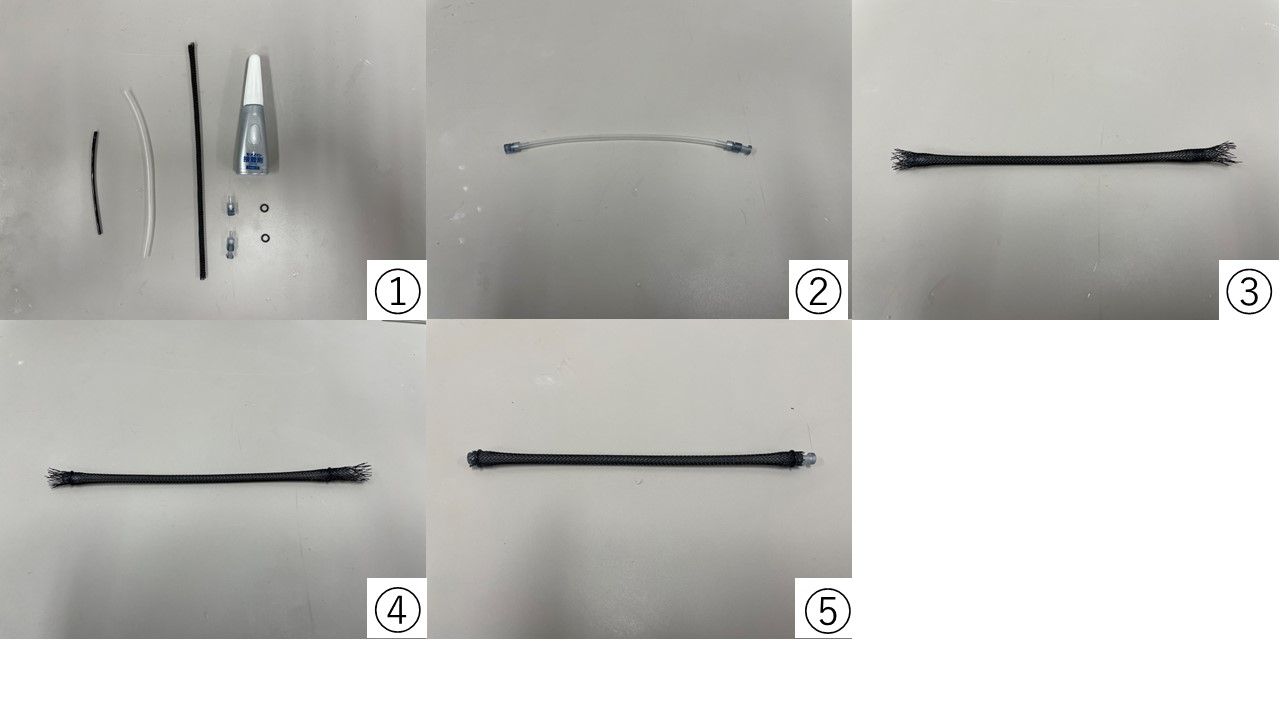
\includegraphics[scale=0.4]{image/sakusei.jpg}
%  \caption{改良型細径MPAの作製方法}
% \label{fig:shingata_sakuseihouhou}
%\end{figure}
%%%%%%%%%%%%%%%%%%%%%%%%%%%%%%%%%%%%%%%%%%%%%%%%%%%%%%%%%

